\documentclass[11pt]{beamer}
\usepackage{color,soul}
\usepackage[utf8]{inputenc}
\usepackage{amsmath}
\usepackage{amsfonts}
\usepackage{amssymb}
\usepackage{algpseudocode} % uses algorithmicx package automatically
\usepackage{mathrsfs}
\usepackage{graphicx}
\usepackage{subcaption}
\DeclareMathOperator*{\argmin}{\mathbf{arg\,min}}
\DeclareMathOperator*{\argmax}{\mathbf{arg\,max}}
%\DeclareMathOperator*{\sup}{sup}
\DeclareMathOperator{\F}{\mathcal{F}} % Function Classes
\DeclareMathOperator{\FF}{\mathcal{F}} % prettier function classes
\DeclareMathOperator{\Hs}{\mathscr{H}} % Hilbert Spaces
\DeclareMathOperator{\R}{\mathbb{R}} % Reals
\DeclareMathOperator{\Rad}{\mathcal{R}} % Rademacher
\DeclareMathOperator{\E}{\mathbb{E}} % Expectation
\DeclareMathOperator{\Or}{\mathcal{O}} % Order Notation
\DeclareMathOperator{\Tr}{\textbf{Tr}} % Expectation
\DeclareMathOperator{\grad}{\nabla} % Gradient
\DeclareMathOperator{\LLH}{\mathcal{L}} % Log Likelihood etc.
\DeclareMathOperator{\Lag}{\mathcal{L}} % Lagrangian etc.
\DeclareMathOperator{\X}{\mathcal{X}} % input space X
\DeclareMathOperator{\Y}{\mathcal{Y}} % output space Y
\DeclareMathOperator{\bF}{\mathbf{F}} 
\DeclareMathOperator{\w}{\mathbf{w}} % weight vector
\DeclareMathOperator{\y}{\mathbf{y}} % output structure
\DeclareMathOperator{\x}{\mathbf{x}} % input structure
\DeclareMathOperator{\f}{\mathbf{f}} % function
\DeclareMathOperator{\K}{\mathcal{K}} % set of Kernels
\DeclareMathOperator{\vw}{\overrightarrow{w}} % set of Kernels
\DeclareMathOperator{\T}{\mathcal{T}} % set of Kernels

%\DeclareMathOperator{\implies}{\rightarrow} % implies

\newcommand{\opt}[1]{{#1}^{*}} % give f* for Optimal, Dual ...
\newcommand{\pred}[1]{\hat{#1}} % Prediction 
\newcommand{\dotprod}[2]{ \langle {#1} , {#2} \rangle } % <w,x> style
\renewcommand{\Pr}{\mathbb{P}} % Probability
\renewcommand{\vec}[1]{\mathbf{#1}} % vectors

\newcommand*{\Let}[2]{\State {#1} $\gets$ {#2}}

\usepackage{xcolor}

\newcommand{\highlight}[1]{\colorbox{yellow}{$\displaystyle #1$}}
\newcommand{\highlightmath}[1]{\colorbox{yellow}{\[\displaystyle #1\]}}


\author{Shyam Upadhyay}
\title{Qualifying Exam}

\setbeamercovered{transparent} 
\date{Shyam Upadhyay} 

\begin{document}

\begin{frame}
\titlepage
\end{frame}

\begin{frame}{About Me}
\begin{itemize}
\item Working with Dan Roth since August 2013.
\item Interested in machine learning and NLP.
\item Publication in AAAI'15 on Learning with Amortized Inference.
\end{itemize}
\end{frame}

\begin{frame}{My Current Research}
Grounding Events to a Knowledge Base
\begin{block}{}
After the {\color{blue} death of \highlightchunk{red}{Cromwell}} in 1658, \highlightchunk{red}{Charles'} chances of regaining the Crown at first seemed slim as Cromwell was succeeded as Lord Protector by his son, Richard.
\end{block}
\end{frame}

\begin{frame}{Motivation}
\begin{itemize}
\item Event mentions in a text demonstrate ambiguity and variability just like named-entities.
\begin{exampleblock}{Variability}
%% \begin{multicols}{2}
%% \begin{itemize}
\emph{Battle of Waterloo, defeat at Waterloo, campaign of Waterloo, the 1815 battle, Napolean's defeat, French cavalry attack}
%% \end{itemize}
%% \end{multicols}
\end{exampleblock}
\begin{exampleblock}{Example for Ambiguity}
\emph{\highlightchunk{red}{At the Olympics} in Athens, Greece, Kupets won a silver medal with her fellow U.S. team members in the team all-around competition.}
\end{exampleblock}
\item Benefits of grounding events - more context available for downstream tasks like event coreference, news aggregation etc.
\end{itemize}
\end{frame}

%% \begin{frame}
%% \end{frame}

%%%%%%%%%%%%%%%%%%%%%%%%%%%%%%%%%%%%%%%%%%%%%%%%%%%%%%%%%%%%
\begin{frame}{Comparison with Entity Wikification}

\begin{itemize}
\item Only 1\% of wikipedia pages are about events. Number higher if you consider events in subheading of an entity's page (eg. ``Invasion of Russia'' section under the wikipage of \textsc{Napolean}).
\item Candidate generation is not as trivial as dictionary look-up.
\pause
\item {\color{red}solution:} Cascaded filtering.
\pause
\item Mentions are not as specific. "Chicago" vs "the civil war".
\pause
\item {\color{red}solution:} Dynamic context expansion.
\end{itemize}
\end{frame}

%%%%%%%%%%%%%%%%%%%%%%%%%%%%%%%%%%%%%%%%%%%%%%%%%%%%%%%%%%%%
\begin{frame}
\begin{block}{Problem}
Candidate generation is not as trivial as dictionary look-up.
\end{block}
\begin{exampleblock}{Possible Solution}
Cascaded filtering
\end{exampleblock}
\begin{block}{Problem}
Mentions are not as specific. "Chicago" vs "the civil war".
\end{block}
\begin{exampleblock}{Possible Solution}
Cascaded filtering
\end{exampleblock}
\end{frame}

\begin{frame}{Premise of the Paper}
\begin{example}
Test
\end{example}
\end{frame}

\begin{frame}{Premise of the Paper}
  %% what is the paper trying to solve
\end{frame}

%%%%%%%%%%%%%%%%%%%%%%%%%%%%%%%%%%%%%%%%%%%%%%%%%%


\begin{frame}
  \begin{center}
    {\huge A* Sampling
    } \\
    Maddison,Tarlow,Minka
  \end{center}
\end{frame}

%%%%%%%%%%%%%%%%%%%%%%%%%%%%%%%%%%%%%%%%%%%%%%%%%%
\begin{frame}{Introduction - Partition Function Woes}
  \begin{itemize}
  \item Gibbs Distribution
    \begin{align*}
      \Pr(\x;\theta) =\frac{\exp(\theta^T\psi(\x))}{Z} \tag{$Z=\sum_{\x} \theta^T\psi(\x)$}
    \end{align*}
  \item ML parameter estimation,
    \begin{align*}
      - \nabla_\theta \log LLH = \E_{\Pr(x;\theta)}\left[\psi(\x)\right] - \frac{1}{T} \sum_i\psi(x_i)
    \end{align*}
  \item   Computing $\E_{\Pr(x;\theta)}[.]$ often intractable.
  % Sampling from posterior is hard
  \item So we resort to approximations. % MCMC, Contrastive Divergence
    %% \item This paper provides a way to obtain exact samples from a intractable distribution.
    %% sampling is inherently tied to Z
    %% but computing Z is #P hard in general
  \end{itemize}
\end{frame}

%%%%%%%%%%%%%%%%%%%%%%%%%%%%%%%%%%%%%%%%%%%%%%%%%%
\begin{frame}<1-3>[label=framelabel]{Detour - Gumbel Distribution}
  Gumbel with location parameter $m$, $Gumbel(m)$.
  \begin{itemize}
    %% & CDF(x;\mu) = \exp \left(-\exp\left(-x+\mu\right)\right) \\
  \item CDF for $Gumbel(m)$, $\Pr(G\le g) = \exp(-\exp(-g+m))$ \\
    \pause
  \item Mean is $m+\gamma$, Variance is $\frac{\pi^2}{6}$.
    \pause
  \item\alert<4->{For $G(i) \sim Gumbel(0)$, and any $B \subseteq [n]$
    \begin{align*}
      & \argmax_{i \in B}{G(i)+\phi(i)} \sim \frac{\exp(\phi(i))}{\sum_{i \in B} \exp(\phi(i))} \\
      & \max_{i \in B}{G(i)+\phi(i)} \sim Gumbel\left(\log \sum_{i \in B} \exp(\phi(i))\right) \tag{Max-Stability}
      %% proof in \cite{hazan}
    \end{align*}
  }
  \end{itemize}
  %% \pause\tikz[overlay,remember picture]{\draw[draw=red,thick,fill opacity=0.2] ($(boxlabel)+(-0.5,0.4)$) rectangle ($(boxlabel)+(11,-4.5)$);}
\end{frame}

%%%%%%%%%%%%%%%%%%%%%%%%%%%%%%%%%%%%%%%%%%%%%%%%%%
%% \begin{frame}{Key Properties}
%% \end{frame}

%%%%%%%%%%%%%%%%%%%%%%%%%%%%%%%%%%%%%%%%%%%%%%%%%%
\begin{frame}{Gumbel-Max Trick (Discrete Case)}
  Suppose you have a discrete distribution specified by un-normalized log probabilities $\{\phi(i)\}_{i=1}^{k}$ over k configurations $\{x_1,\cdots,x_k\}$, i.e.,
  \begin{align}
    \Pr(x_i) = \frac{\exp\phi(i)}{\sum_j\exp\phi(j)} \label{eq:gibbs}
  \end{align}
  We can draw samples $x_i \sim \Pr$ from this distribution using the following procedure.
  \begin{align*}
    & \text{Sample} \qquad G(i) \sim Gumbel(0) \text{ for } i=1..k\\
    & \text{then} \qquad \text{ Choose } x_j \text{ such that } j= \argmax_i \{G(i) +\phi(i)\} \tag{the argmax of the perturbed probabilities is distributed as eq.\ref{eq:gibbs} above}
  \end{align*}

\end{frame}
\againframe<4>{framelabel}
%%%%%%%%%%%%%%%%%%%%%%%%%%%%%%%%%%%%%%%%%%%%%%%%%%
\begin{frame}{Benefits} %{Wait ... So What?}
  %% All this is cute, but what is the benefit?
  \begin{itemize}
  \item Partition Function evaluation $\implies$ Computing (many) perturbed MAPs. % We have reduced a to b. No need to compute the partition function, as long as you can compute the (perturbed) argmax!
  \item \emph{Exact} samples from the target distribution. % Note that the samples are exact. (No approximations!)
    %(examples when things are approximations, MCMC ``once the chain reaches stationary distribution'')
  \end{itemize}
  But ...
  \begin{itemize}
  \item What happens if we move from discrete to continuous space?
  \item \textsc{Question:} Is There A Gumbel Max Trick for Continuous Distributions? %% One that does not resort to making infinite??exponential perturbations?
    \pause
  \item {\color{red} This paper --- Yes!}
  \end{itemize}
\end{frame}

%% %%%%%%%%%%%%%%%%%%%%%%%%%%%%%%%%%%%%%%%%%%%%%%%%%%
%% \begin{frame}{Gumbel and the Partition Function}
  
%% \end{frame}

%%%%%%%%%%%%%%%%%%%%%%%%%%%%%%%%%%%%%%%%%%%%%%%%%%
\begin{frame}{Perturbing Gumbel Process Variates}
  %% just put image
  For $B \subseteq \Omega$,
  \begin{align*}
  \max \{G_k \mid X_k \in B\} \sim Gumbel(log \mu(B)) \\
  \argmax \{G_k \mid X_k \in B\} \sim \frac{\exp(\phi(x))1_{x \in B}}{\mu(B)} \\
  \end{align*}
  Then $\{ \max \{G_k \mid X_k \in B\} \mid B \subseteq \Omega\}$ is a Gumbel Process.
\end{frame}

%% %%%%%%%%%%%%%%%%%%%%%%%%%%%%%%%%%%%%%%%%%%%%%%%%%%
%% \begin{frame}{High Dimensional Sampling is Exponential}

%% \end{frame}

%%%%%%%%%%%%%%%%%%%%%%%%%%%%%%%%%%%%%%%%%%%%%%%%%%
\begin{frame}{Main Idea}
  \emph{We can transform a Gumbel process into another by adding the difference of their log densities.} \\
  \begin{align*}
  & \mu(B) = \int_{x\in B} \exp(\phi(x)) \\
  & \nu(B)=\int_{x\in B} \exp(i(x)) \\
  & \text{ Let $o(x) = \phi(x) - i(x)$ be bounded} \\
  & \{\{G_k + o(X_k) \mid X_k \in B\} \mid B \subseteq \R^d\} \text{ is a Gumbel Process with measure $\mu$}
  \end{align*}
   
  %% So if I can easily draw samples from the prior and I have a way to compute the bound on the log-likelihood, then I can use Gumbel.
\end{frame}
\begin{frame}{Progress So Far}
  \begin{itemize}
  \item We wanted to draw samples from target distribution.
  \item We reduced it to computing argmax of a sequence of samples from a exotic distribution. (because argmax follows the target dist)
  \end{itemize}
  Problems
  \begin{itemize} 
  \item Drawing samples from the distribution requires knowing Z of my target distribution.
  \item We do not want to draw infinite samples to compute argmax on.
  \end{itemize}
  Solutions
  \begin{itemize} 
  \item I can draw samples from easier distribution, because I know its log Z. and then add the hard part to the samples before taking argmax.
  \item Do A* search.
  \end{itemize}
\end{frame}

%%%%%%%%%%%%%%%%%%%%%%%%%%%%%%%%%%%%%%%%%%%%%%%%%%
\begin{frame}{Top-Down Construction of Gumbel Process}
  Assume log Z is computable for now.
\end{frame}



\begin{frame}{Main Idea}
  \centering
  \begin{tikzpicture}[scale=0.8]
    %% \draw[step=0.5,gray] (-5,-5) grid (5,5);
    \draw[ultra thick,gray] plot[smooth] coordinates {(-6,0)(-5,0)(-3,3) (0,-1) (3,3) (5,0)};
    \node (ox) at (-4,-1) {o(x)};

    %% \begin{axis}[height=10cm,width=10cm]
    %%   \addplot[ultra thick,gray,smooth] coordinates {
    %%     (-6,0)(-5,0)(-3,3) (0,-1) (3,3) (5,0)}
    %%   node [pos=0.9,below left] {o(x)};
    %% \end{axis}
    
    \only<2>{
      \path[draw,dotted,blue,very thick] (-5,5) -- (5,5);
    }
    %% \addplot+[ycomb,black,thick] {1};
    %% \node[above] (g1) at (0,4) {};

    \onslide<2->{
      \path[draw,red,thick] (0,-1) -- (0,4) circle (1.5pt);
      \node[above] at (0,4.25) {$g_1+o(x_1)$};
    }
    
    \only<2,3>{
      \path[draw,green,dotted,very thick] (-5,4) -- (5,4);
    }
    
    \onslide<3->{
      \path[draw,red,thick] (-3,3) -- (-3,2) circle (1.5pt);
      \node[below] at (-3,1.5) {$g_2+o(x_2)$};
    }

    \only<3,4,5>{
      \path[draw,dotted,blue,very thick] (-5,3.5) -- (0,3.5);
    }
    
    \onslide<4->{
      \path[draw,red,thick] (3,3) -- (3,4.5) circle (1.5pt);
      \node[below] at (3,5.25) {$g_3+o(x_3)$};
    }
    \only<3->{
      \path[draw,dotted,blue,very thick] (0,5) -- (5,5);
    }
    \only<4->{
      \path[draw,green,dotted,very thick] (-5,4.5) -- (5,4.5);
    }
  \end{tikzpicture}  
\end{frame}

\begin{frame}
  But
\end{frame}



\begin{frame}[allowframebreaks]{References}
\def\newblock{}
\bibliographystyle{apalike}
\bibliography{quals.bib}
\end{frame}

\end{document}
